\documentclass[12pct,twoside, openright]{report}
%\usepackage[hmarginratio=1:1,top=3cm,bottom=3cm]{geometry}
\usepackage[a4paper,inner=3.5cm,outer=2.5cm,top=3.5cm,bottom=4.5cm,pdftex]{geometry}
\usepackage{minitoc}
\usepackage{listings}  
\lstset{language=matlab,
	backgroundcolor=\color{gray!20}} 
\usepackage{emptypage}
\usepackage{makeidx}
\usepackage{etoolbox,ragged2e,siunitx}
\usepackage{pdfpages}
\usepackage{capt-of}
%\usepackage[colorinlistoftodos, shadow]{todonotes}
\usepackage[textwidth=1.5cm]{todonotes}
\setlength{\marginparwidth}{1.5cm}

\usepackage[utf8]{inputenc}


%\usepackage[ansinew]{inputenc}										% Gør det muligt at bruge æ, ø og å i sine .tex-filer
\usepackage[T1]{fontenc}
\usepackage[english]{babel}
\usepackage{amsmath , amsfonts , amssymb}
 \numberwithin{equation}{section}
%\usepackage[hmargin=3cm,vmargin=3.5cm]{geometry}
\usepackage{multirow}
\usepackage{graphicx}
\usepackage{epstopdf}
\usepackage[hang,bf]{caption}
%\usepackage[usenames,dvipsnames]{xcolor}
\usepackage{subcaption}
\usepackage[authoryear]{natbib} 
%\usepackage[numbers]{natbib} 
\bibliographystyle{apalike}
%\bibliographystyle{abbrvnat} 
%\usepackage{lipsum}\usepackage{blindtext}
\usepackage{wrapfig}
\usepackage[absolute]{textpos}
\usepackage{graphicx}
\usepackage{pgfplotstable}
\usepackage{pgfplots}
\usepackage{xcolor,colortbl}
%\usepackage{gnuplot-lua-tikz}
\usepackage{lipsum}
\usepackage{color}
\usepackage{lastpage}
\usepackage{float}
\usepackage{fancyhdr}
\usepackage[bookmarks=true , bookmarksopen=true,bookmarksnumbered=true,pagebackref=true,colorlinks=blue,breaklinks=true]{hyperref}
\usepackage{array}
\usepackage{rotating}
\usepackage[titletoc]{appendix}
\usepackage{tikz}
\usetikzlibrary{arrows,decorations.markings, plotmarks,shapes}
%\usetikzlibrary{arrows.meta}
\usetikzlibrary{intersections}
\usepackage{tkz-euclide}
\usetkzobj{all}

\usepackage[europeanresistors,americaninductors]{circuitikz}
\usepackage[Lenny]{fncychap}




\ChNameVar{\fontsize{14}{16}\usefont{OT1}{phv}{m}{n}\selectfont}
\ChNumVar{\fontsize{60}{62}\usefont{OT1}{ptm}{m}{n}\selectfont}
\ChTitleVar{\centering\Huge\bfseries\rm}
\ChRuleWidth{1pt}

\fancypagestyle{plain}{%
  \renewcommand{\headrulewidth}{0pt}%
 \fancyhf{}%
  \fancyfoot[OR]{\thepage\ af \pageref{LastPage}}
  \fancyfoot[EL]{\thepage\ af \pageref{LastPage}}%
}
%\fancypagestyle{fancy}{%
%  \renewcommand{\headrulewidth}{0pt}%
% \fancyhf{}%<path to your tex file>\yourtexfile.nlo -s nomencl.ist -o <path to your tex file>\yourtexfile.nls
%  \fancyfoot[OR]{\footnotesize Side \thepage\ af \pageref{LastPage}}
%  \fancyfoot[EL]{\footnotesize Side \thepage\ af \pageref{LastPage}}%
%}
\pagestyle{fancy}

\lhead{4.119f}
\chead{\leftmark}
\rhead{\today}
\cfoot{}
\fancyfoot[OR]{\thepage\ af \pageref{LastPage}}
\fancyfoot[EL]{\thepage\ af \pageref{LastPage}}

\renewcommand{\headrulewidth}{0.4pt}
\renewcommand{\footrulewidth}{0.4pt}
\newcommand*{\tomlinje}[0]{\\[\baselineskip]
   \setlength{\parskip}{0pt}}
\newcommand{\mat}[1]{\left[\begin{matrix}
#1
\end{matrix}	\right]}
\newcommand{\vect}[1]{\left\{\begin{matrix}
#1
\end{matrix}    \right\}}
\newcommand{\kapitel}{./Kapitler/Kapitel_2_produktanalyse/}
\newcommand{\HRule}{\rule{\linewidth}{0.5mm}}
\addto\captionsdanish{
\renewcommand\appendixname{Appendiks}
\renewcommand\contentsname{Indholdsfortegnelse}}
\definecolor{green}{rgb}{.55,0.75,0}


\usepackage[firstpage]{draftwatermark}
%\SetWatermarkLightness{2}
%\SetWatermarkText{\includegraphics[height=\textheight , width=\textwidth , angle = -45]{./billeder/aau_waves_3}}


\graphicspath{
{./billeder/},
{./billeder/problem_analysis/},
{./billeder/modeling/},
{./billeder/vision/},
}




\newcommand{\ind}{./afsnit/introduction/}
\newcommand{\g}{\,}
\newcommand{\T}[2]{{^{#1} A_{#2}}}


\begin{document}
\section{læsevejledning}
\begin{itemize}
  \item Preface skal der blot ses bort fra
  \item Jeg har lavet en indholdsfortegnelse over hvad jeg forstiller mig raporten skal indeholde
  \item Kapitel 1, introduktion: Jeg har ikke skrevet det i nu, men forestiller mig at skrive noget med robotter i produktionen generelt og slutte den af med et initierende problem
  \item Kapitel 2: problem analysis, Det hele er klar til gennemlæsning og vil gerne have feedback omkring indhold, den røde tråd osv. 
  \item kapitel 3: Udkast til problemformulering, hvad synes I? derudover tænker jeg der skal laves en afgrænsning 

\end{itemize}


\pagenumbering{roman}
\setcounter{page}{1}
%\includegraphics[width=\textwidth]{./forside/Forside}
\begin{titlepage}

\newgeometry{left=1cm, right = 1cm, bottom = 1cm, top = 1cm }
\enlargethispage{10\baselineskip}
%\newcommand{\HRule}{\rule{\linewidth}{0.5mm}} % Defines a new command for the horizontal lines, change thickness here



\center % Center everything on the page
 
%----------------------------------------------------------------------------------------
%	HEADING SECTIONS
%----------------------------------------------------------------------------------------

\begin{minipage}[t]{\textwidth}
%\vspace{0cm}
\begin{flushright}
  

\includegraphics[scale=1]{./forside/84800_aau_uk_studentreport_blue_cmyk}
\end{flushright}

\end{minipage}\\[1cm]
%\textsc{\LARGE Aalborg University}\\[1.5cm] % Name of your university/college
\HRule \\[0.4cm]
{ \huge \bfseries Visual Servoing of SCARA Adept Robot}\\[0.2cm] % Title of your document
\HRule \\[.4cm]
%\textsc{\Large Major Heading}\\[0.5cm] % Major heading such as course name
%\textsc{\large Minor Heading}\\[0.5cm] % Minor heading such as course title

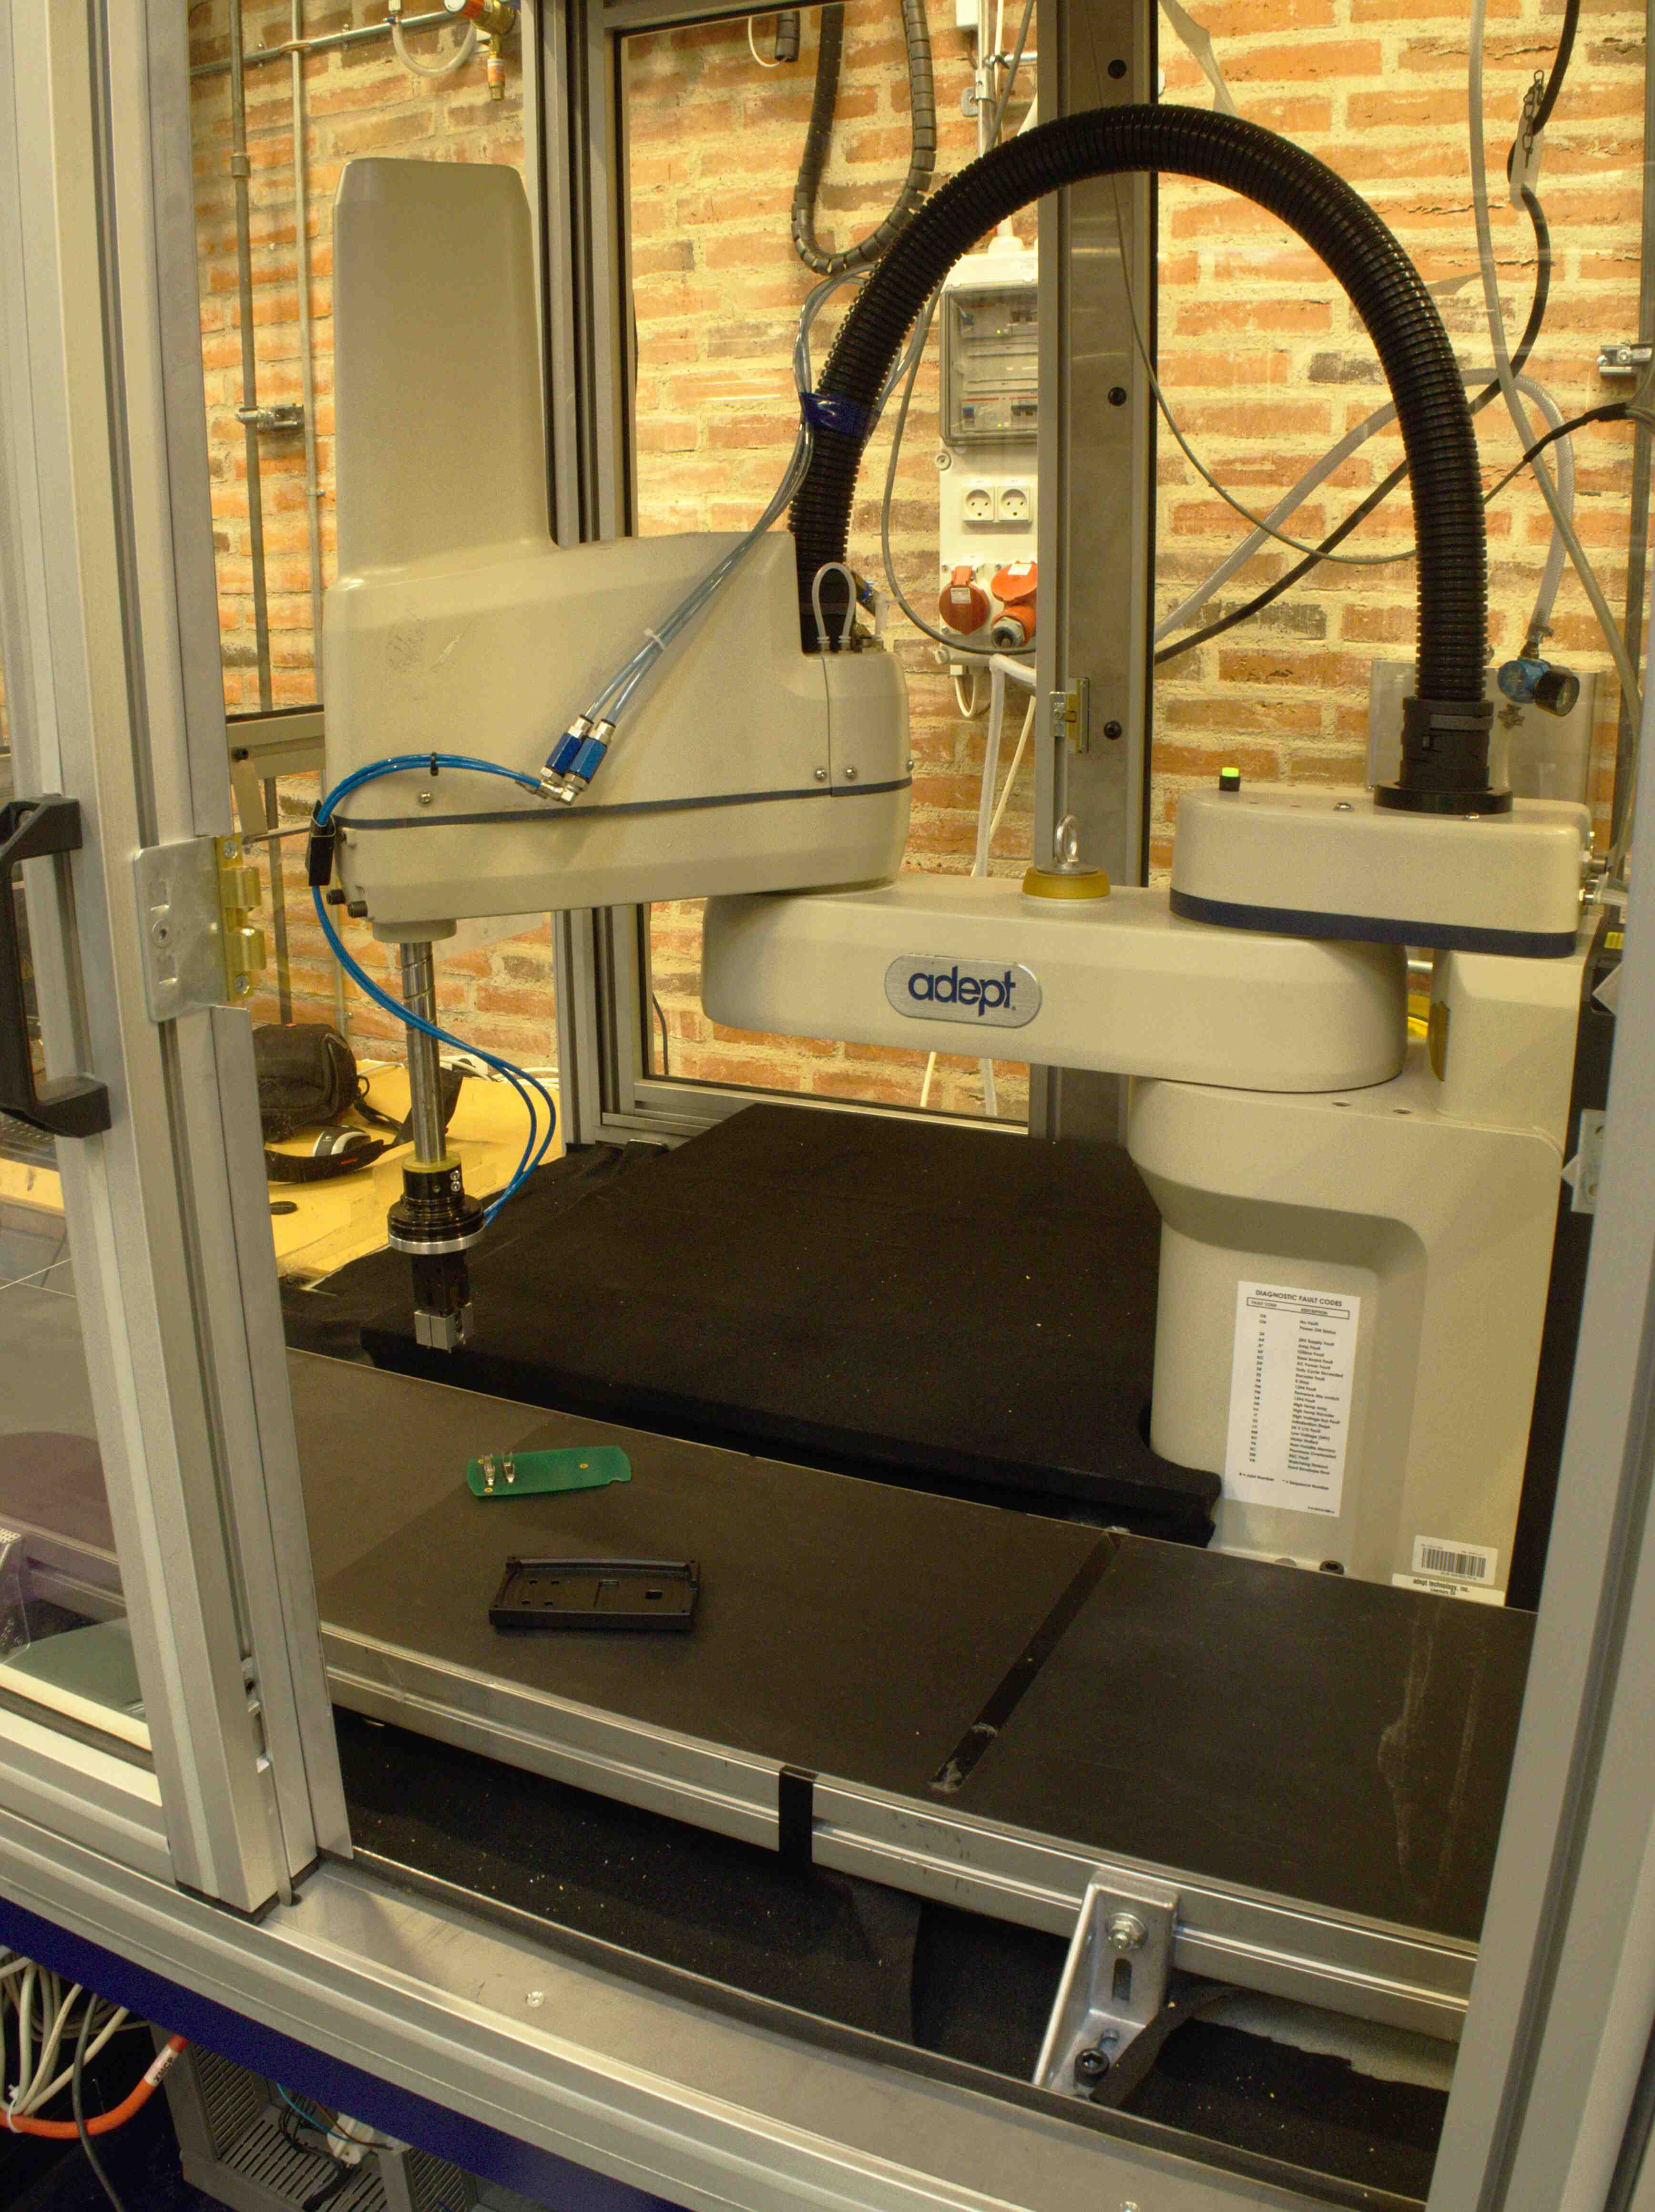
\includegraphics[width=0.6\textwidth]{./forside/fronpage_test}
\\[0.4cm]
\HRule \\[0.4cm]
{ \bfseries Master Thesis }\\[0.2cm] % Title of your document
\HRule \\[.4cm]
%----------------------------------------------------------------------------------------
%	TITLE SECTION
%----------------------------------------------------------------------------------------

\vspace{1cm}
 
%----------------------------------------------------------------------------------------
%	AUTHOR SECTION
%----------------------------------------------------------------------------------------



\begin{center}


\begin{tabular}{l p{5cm} l}


   
    \large \colorbox{white!30}{\emph{Author:}} && \large \colorbox{white!30}{\emph{Supervisor:}}\\[0.1cm]
   \large \colorbox{white!30}{Thomas Pank \textsc{Roulund}} && \large  \colorbox{white!30}{Ole \textsc{Madsen}} \\
     && \large  \colorbox{white!30}{Rasmus Skovgaard \textsc{Andersen}} \\
  
    
   
\end{tabular}
\end{center}
%\begin{minipage}{\textwidth}
%\begin{flushleft}\emph{Authors:}\end{flushleft}\begin{flushright}\emph{Supervisor:}\end{flushright}
%Klaus Bro \textsc{Jensen} \\
%Max Møller \textsc{Madsen}\\
%Chris Skaarup \textsc{Ahle}\\
%Thomas Pank \textsc{Roulund}
%
%\end{minipage}
%~
%\begin{minipage}{0.4\textwidth}
%\begin{flushright} \large
%\emph{Supervisor:} \\[0.1cm]
%Christian \textsc{Nørgaard}\\
%%Mikkel Melters \textsc{Pedersen} % Supervisor's Name
%\end{flushright}
%\end{minipage}\\[1cm]

% If you don't want a supervisor, uncomment the two lines below and remove the section above
%\Large \emph{Author:}\\
%John \textsc{Smith}\\[3cm] % Your name

%----------------------------------------------------------------------------------------
%	DATE SECTION
%----------------------------------------------------------------------------------------

%{\large \today} % Date, change the \today to a set date if you want to be precise

%----------------------------------------------------------------------------------------
%	LOGO SECTION
%----------------------------------------------------------------------------------------

%\includegraphics{Logo}\\[1cm] % Include a department/university logo - this will require the graphicx package
 
%----------------------------------------------------------------------------------------

\vfill % Fill the rest of the page with whitespace

\end{titlepage}

\clearpage
\restoregeometry
\thispagestyle{empty}
\newpage
\mbox{}
\clearpage

%\documentclass[12pct,twoside, openright]{report}
%\usepackage[hmarginratio=1:1,top=3cm,bottom=3cm]{geometry}
\usepackage[a4paper,inner=3.5cm,outer=2.5cm,top=3.5cm,bottom=4.5cm,pdftex]{geometry}
\usepackage{minitoc}
\usepackage{listings}  
\lstset{language=matlab,
	backgroundcolor=\color{gray!20}} 
\usepackage{emptypage}
\usepackage{makeidx}
\usepackage{etoolbox,ragged2e,siunitx}
\usepackage{pdfpages}
\usepackage{capt-of}
%\usepackage[colorinlistoftodos, shadow]{todonotes}
\usepackage[textwidth=1.5cm]{todonotes}
\setlength{\marginparwidth}{1.5cm}

\usepackage[utf8]{inputenc}


%\usepackage[ansinew]{inputenc}										% Gør det muligt at bruge æ, ø og å i sine .tex-filer
\usepackage[T1]{fontenc}
\usepackage[english]{babel}
\usepackage{amsmath , amsfonts , amssymb}
 \numberwithin{equation}{section}
%\usepackage[hmargin=3cm,vmargin=3.5cm]{geometry}
\usepackage{multirow}
\usepackage{graphicx}
\usepackage{epstopdf}
\usepackage[hang,bf]{caption}
%\usepackage[usenames,dvipsnames]{xcolor}
\usepackage{subcaption}
\usepackage[authoryear]{natbib} 
%\usepackage[numbers]{natbib} 
\bibliographystyle{apalike}
%\bibliographystyle{abbrvnat} 
%\usepackage{lipsum}\usepackage{blindtext}
\usepackage{wrapfig}
\usepackage[absolute]{textpos}
\usepackage{graphicx}
\usepackage{pgfplotstable}
\usepackage{pgfplots}
\usepackage{xcolor,colortbl}
%\usepackage{gnuplot-lua-tikz}
\usepackage{lipsum}
\usepackage{color}
\usepackage{lastpage}
\usepackage{float}
\usepackage{fancyhdr}
\usepackage[bookmarks=true , bookmarksopen=true,bookmarksnumbered=true,pagebackref=true,colorlinks=blue,breaklinks=true]{hyperref}
\usepackage{array}
\usepackage{rotating}
\usepackage[titletoc]{appendix}
\usepackage{tikz}
\usetikzlibrary{arrows,decorations.markings, plotmarks,shapes}
%\usetikzlibrary{arrows.meta}
\usetikzlibrary{intersections}
\usepackage{tkz-euclide}
\usetkzobj{all}

\usepackage[europeanresistors,americaninductors]{circuitikz}
\usepackage[Lenny]{fncychap}




\ChNameVar{\fontsize{14}{16}\usefont{OT1}{phv}{m}{n}\selectfont}
\ChNumVar{\fontsize{60}{62}\usefont{OT1}{ptm}{m}{n}\selectfont}
\ChTitleVar{\centering\Huge\bfseries\rm}
\ChRuleWidth{1pt}

\fancypagestyle{plain}{%
  \renewcommand{\headrulewidth}{0pt}%
 \fancyhf{}%
  \fancyfoot[OR]{\thepage\ af \pageref{LastPage}}
  \fancyfoot[EL]{\thepage\ af \pageref{LastPage}}%
}
%\fancypagestyle{fancy}{%
%  \renewcommand{\headrulewidth}{0pt}%
% \fancyhf{}%<path to your tex file>\yourtexfile.nlo -s nomencl.ist -o <path to your tex file>\yourtexfile.nls
%  \fancyfoot[OR]{\footnotesize Side \thepage\ af \pageref{LastPage}}
%  \fancyfoot[EL]{\footnotesize Side \thepage\ af \pageref{LastPage}}%
%}
\pagestyle{fancy}

\lhead{4.119f}
\chead{\leftmark}
\rhead{\today}
\cfoot{}
\fancyfoot[OR]{\thepage\ af \pageref{LastPage}}
\fancyfoot[EL]{\thepage\ af \pageref{LastPage}}

\renewcommand{\headrulewidth}{0.4pt}
\renewcommand{\footrulewidth}{0.4pt}
\newcommand*{\tomlinje}[0]{\\[\baselineskip]
   \setlength{\parskip}{0pt}}
\newcommand{\mat}[1]{\left[\begin{matrix}
#1
\end{matrix}	\right]}
\newcommand{\vect}[1]{\left\{\begin{matrix}
#1
\end{matrix}    \right\}}
\newcommand{\kapitel}{./Kapitler/Kapitel_2_produktanalyse/}
\newcommand{\HRule}{\rule{\linewidth}{0.5mm}}
\addto\captionsdanish{
\renewcommand\appendixname{Appendiks}
\renewcommand\contentsname{Indholdsfortegnelse}}
\definecolor{green}{rgb}{.55,0.75,0}


\usepackage[firstpage]{draftwatermark}
%\SetWatermarkLightness{2}
%\SetWatermarkText{\includegraphics[height=\textheight , width=\textwidth , angle = -45]{./billeder/aau_waves_3}}

%\begin{document}


\enlargethispage{20em}


\begin{titlepage}
\setcounter{page}{1}
\thispagestyle{plain}
\begin{samepage}
{\samepage 
\begin{tabular}{r}
\parbox{\textwidth}{  \raisebox{9mm}{
\includegraphics{./forside/84800_aau_uk_studentreport_blue_cmyk}}
\hfill \parbox{6.7cm}{\begin{tabular}{l}
{\sf\small \textbf{http://www.m-tech.aau.dk/}} \\
{\sf\small  \textbf{Electro-Mechanical System Design}} \\
{\sf\small Fibigerstræde 16} \\
{\sf\small Telefon 99 40 71 17} \\
{\sf\small Fax 99 40 71 10} \\
{\sf\small http://info@m-tech.aau.dk}
\end{tabular}}}
\\
\end{tabular}

\begin{tabular}{cc}
\parbox{7cm}{
\begin{description}

\item {\bf Title:} 

Vision Control of SCARA Adept robot and planning of pick and place operation
  
\item {\bf Theme:} 

Master Thesis 

\end{description}

\parbox{8cm}{

\begin{description}
\item {\bf Project period:}\\
   P10, EMSD4\\
  \hspace{4cm}
\item {\bf Project group:}\\
  4.119f\\
  \hspace{4cm}
\item {\bf Authors:}

Thomas Pank Roulund \\
\item {\bf  Supervisors:}\\[0.5em]
 Ole Madsen  \\[0.5em]
 Rasmus Skovgaard Andersen  \\[0.5em]
 
  \end{description}
}
\begin{description}
\item {\bf Printed copies: x} 
\item {\bf Pages: x} 
\item {\bf x annex and x appendix} 
\item {\bf Completed: 18.12.2015} 
\end{description}
\vfill } &
\parbox{7cm}{
  \vspace{.15cm}
  \hfill 
  \begin{tabular}{l}
  {\bf Synopsis:}\bigskip \\
  \fbox{
    \parbox{6.5cm}{\bigskip
     {\vfill{\small %This project covers the design and control of a load system. The load system's purpose is to test linear actuators against linear and non-linear loads. This requires a system with a test actuator and an active actuator to emulate different loads. First an initial design was made on these terms. The initial design became final by designing against static and fatigue loads, specified by the costumer, using Eurocode 3, Norton for bolt assemblies and Schaeffler's own method for the bearings. \newline
%Finally a mechanical- and hydraulic model were made and implemented in Simulink to simulate the load system by making a kinematic and kinetic analysis of the mechanical system and a dynamic analysis of the hydraulic system. The validation of the dynamic model concluded, that it is necessary to design controllers for the dynamic model to meet the design criteria. The dynamic model was transformed into a linear model, which was used to design two PID-controllers by analysing the bode plots for the transfer functions. These controllers where implemented in the dynamic model together with a saturation on the controller output signal making it necessary to implement an anti wind up loop.\newline
%The designed load system has necessary strength and service life to fulfil the design criteria and the designed controllers for the dynamic model of the load system makes the load system fulfil the dynamic requirements to the load system. In conclusion the project has been a success because all the design criterion have been fulfilled.

     \bigskip}}
     }}
   \end{tabular}}
\end{tabular}}
\\ \\

\end{samepage}
\end{titlepage}
%\end{document}
 \clearpage

\clearpage
\chapter*{Preface}
This 4th semester master thesis has been written a student attending the Electro-Mechanical System Design engineering line at Aalborg University. The project period spans from the 2nd of February to the 2nd of June. \newline

%\noindent The project has been made in collaboration with Aalborg Universty since the skateboard has some commercial value at different events. The project makes an analysis of the old project, which leads to some aspects a new design should improve. This includes a new improved design of the skateboard, and a more complex model of the skateboard. Lastly the project designs and implements a controller which stabilizes the skateboard, and is able to verify the model of the skateboard.\newline
\noindent The references are created based on the Harvard method, meaning that each reference is written with both author and year of publish. All figures are named X.Y, where X shows the coherent chapter and Y the figure number. Whenever a table or figure is used a describing text follows to explain the context. If the figure doesn't include a reference its made by the group itself. The chapters in the annex and appendix are written with letters to differentiate between main matter and attachments.\newline
\noindent A CD will be attached to the printed project, including the annex, appendix and all SolidWorks parts with drawings. The drawings are also printed and assembled in a separate holder, to provide easy accessibility for the reader.\newline
\textbf{Software}
The following software has been used in the process of making this project.

\begin{center}

\begin{tabular}{l l |l l}
\hline 
\textbf{Name} & \textbf{Area of use} & \textbf{Name} & \textbf{Area of use}\\ 
\hline  
\LaTeX & Assembling the project & SolidWorks & 3D drawing of the skateboard \\ 
\hline 
Maple 16 & Calculations & Ansys & FE analysis \\ 
\hline 
Matlab & Calculations and scripts & Eagle & Circuit drawing of PCB\\ 
\hline

\end{tabular} \\[2cm]

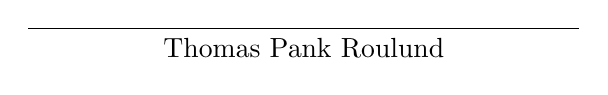
\begin{tikzpicture}[auto]
\draw (0,-1) --node[below]{Thomas Pank Roulund} (7,-1);
\end{tikzpicture}
\end{center}


\clearpage
 \setcounter{tocdepth}{1}
 \tableofcontents 
\clearpage

% %%Nomenclature
% \input{./nomenclature/nomenclature}\clearpage
% 



\thispagestyle{empty}
\newpage
\mbox{}
\clearpage
%\thispagestyle{empty}
%\newpage
%\mbox{}
%\clearpage


\pagenumbering{arabic}
\setcounter{page}{1}

%% Introduction
\renewcommand\ind{./afsnit/introduction/}
\input{\ind introduction}

%% Problem analysis 
\renewcommand\ind{./afsnit/problemanalysis/}
\input{\ind prob_ana_intro}\clearpage
  %section: test setup
  \input{\ind prob_ana_test_setup}\clearpage
  %section: solution strategy
  \input{\ind prob_ana_solution_strategy}\clearpage

%% Problem statement
\renewcommand\ind{./afsnit/problem_statement/}
\input{\ind prob_statement}

%% Vision system
\renewcommand\ind{./afsnit/vision_system/}
\input{\ind vision_system}
\input{\ind image_procesing}

%% Modeling
\renewcommand\ind{./afsnit/modeling/}
\input{\ind modeling}\clearpage
\input{\ind kinematics}\clearpage
\input{\ind housing_model}

\renewcommand\ind{./afsnit/solution_iterations/}
\input{\ind solution_iteration}

%% TO DO REMEMBER TO COMMENT WHEN DONE
\clearpage
\listoftodos
\clearpage

\bibliography{kilder}
\addcontentsline{toc}{chapter}{bibliography}

\appendix
\renewcommand\appendixname{Annex}
\renewcommand\ind{./annex/}
\begin{appendices}
\input{\ind david_hartenberg}
\end{appendices}

\renewcommand\appendixname{Appendix}
\renewcommand\ind{./appendix/}
\begin{appendices}\setcounter{chapter}{0}

\end{appendices}

\end{document}
